\documentclass[tikz,border=2pt]{standalone}
\usepackage{tikz}
\begin{document}
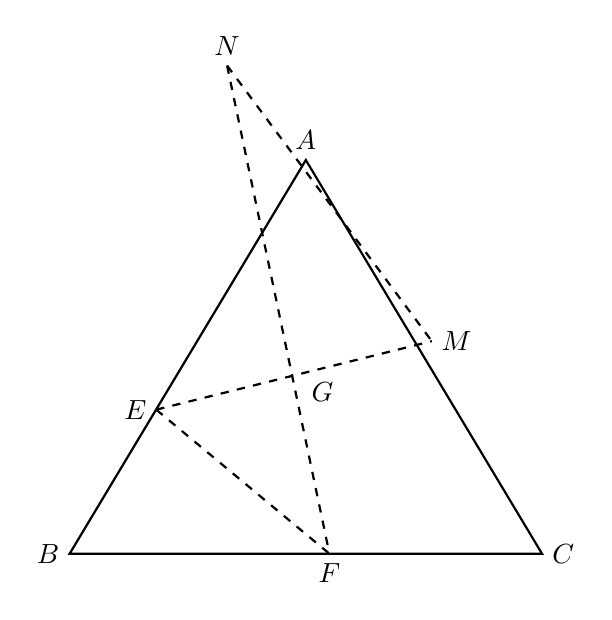
\begin{tikzpicture}[scale=1]

% Triangle
\draw[thick] (0,0) node[left] {$B$} -- (3,5) node[above] {$A$} -- (6,0) node[right] {$C$} -- cycle;

% Point F on BC
\coordinate (F) at (3.3,0);
\node[below] at (F) {$F$};

% Point E on BA
\coordinate (E) at (1.1,1.83);
\node[left] at (E) {$E$};

% Point M on AC (label only, no segment AM)
\coordinate (M) at (4.6,2.7);
\node[right] at (M) {$M$};

% Point N above A
\coordinate (N) at (2.0,6.2);
\node[above] at (N) {$N$};

% Dashed lines
\draw[dashed,thick] (N) -- (F);
\draw[dashed,thick] (N) -- (M);
\draw[dashed,thick] (E) -- (F);
\draw[dashed,thick] (E) -- (M);

% Point G at intersection area
\coordinate (G) at (2.95,2.05);
\node[right] at (G) {$G$};

\end{tikzpicture}
\end{document}
